\documentclass[11pt]{beamer}

%%%%%%%% teme %%%%%%%%
\mode<presentation> {
\usetheme{Madrid}
%\usecolortheme{albatross}
}
\beamertemplatenavigationsymbolsempty
%\usepackage[french]{babel}
\usepackage[utf8]{inputenc}
\usepackage{graphicx} 
\usepackage{booktabs} 
\usepackage[T1]{fontenc}
\usepackage{tikz}

%\usetikzlibrary{decorations}
\usetikzlibrary{decorations.pathreplacing}
\usetikzlibrary{patterns}

\usepackage{minted}
\usepackage{epigraph}
\usepackage{cellspace}
\usepackage{multirow}
\usetikzlibrary{patterns}
\usepackage{amssymb, amsmath, amsfonts, amscd}
\usepackage[noend]{algpseudocode}


\institute[SU] 
{
%================= logos no meio =====================
\vspace*{-0.35cm}

\includegraphics[height=2cm]{pictures/su_logo.png}\hspace{5mm}

\includegraphics[height=2cm]{pictures/cnrs.jpg}\hspace{5mm}

\includegraphics[height=2cm]{pictures/LIP6.png}
\vspace*{0.35cm}\\
%Sorbonne Université - Faculté de Sciences et Ingénierie\\
%\medskip
%\texttt{\{lods.eng,ronety\}@uea.edu.br} % emails
}
\date{\today}
%%% Local Variables:
%%% mode: latex
%%% TeX-master: "main"
%%% End:


%%%%%%%% titre %%%%%%%%
\title[Seed-Recovery for PCG]{Practical Seed-Recovery for the \\ PCG Pseudo-Random Number Generator}

%%%%%%%% noms des auteurs %%%%%%%%
\author[Bouillaguet, Martinez, Sauvage]{
Charles Bouillaguet, Florette Martinez and \alert{Julia Sauvage}} 

%\includeonlyframes{hard_big_cvp}

\begin{document}



\begin{frame}
\titlepage 

\end{frame}

%\begin{frame}
%\frametitle{Contenu} 
%\tableofcontents 
%\end{frame}

%%%%%%%% slides %%%%%%%%
\section{Introduction}
\begin{frame}<1>[label=intro]{Introduction}
    
    \begin{exampleblock}{What?}
        Cryptanalysis of the \textbf{Permuted Congruential Generator} (PCG).
    \end{exampleblock}
    
    \medskip\pause
    
    \begin{alertblock}{Results}
      \textbf{Practical seed-recovery} / prediction.
    \end{alertblock}
    
    \begin{block}{How?}
    \begin{itemize}
        \item "Guess-and-Determine" attack.
        \item Most expensive part : many small CVP problems.
        \item \textbf{Actually done} in $\leq$ 20 000 CPU-hours.
    \end{itemize}  
    \end{block}
\end{frame}

\begin{frame}{Why?}
    \centering
    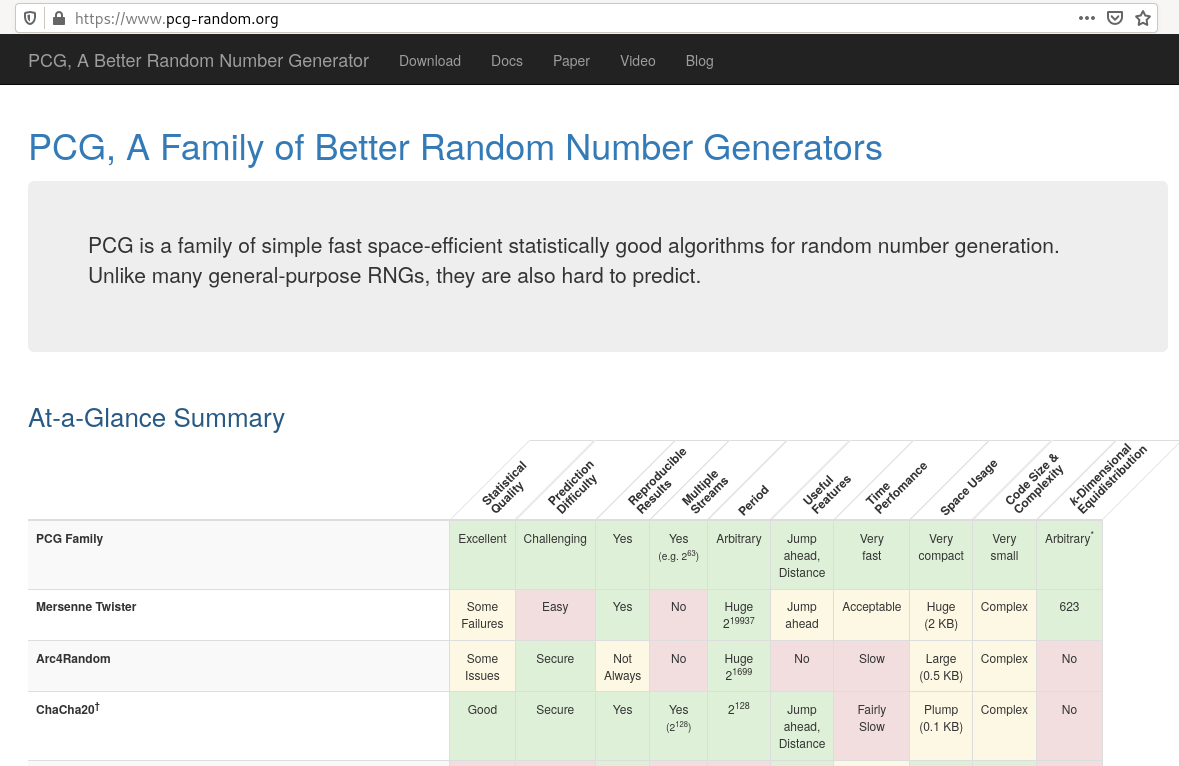
\includegraphics[width=\textwidth]{pictures/website.png}
\end{frame}

\begin{frame}{Why?}
    \centering
    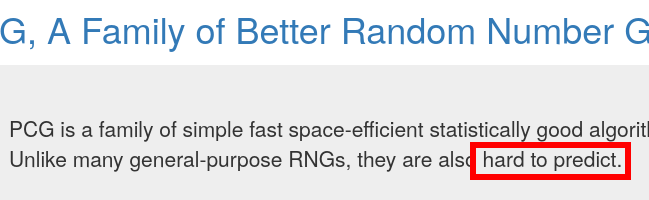
\includegraphics[width=\textwidth]{pictures/hard.png}
    \vfill
  \end{frame}

\begin{frame}{Why?}
    \centering
    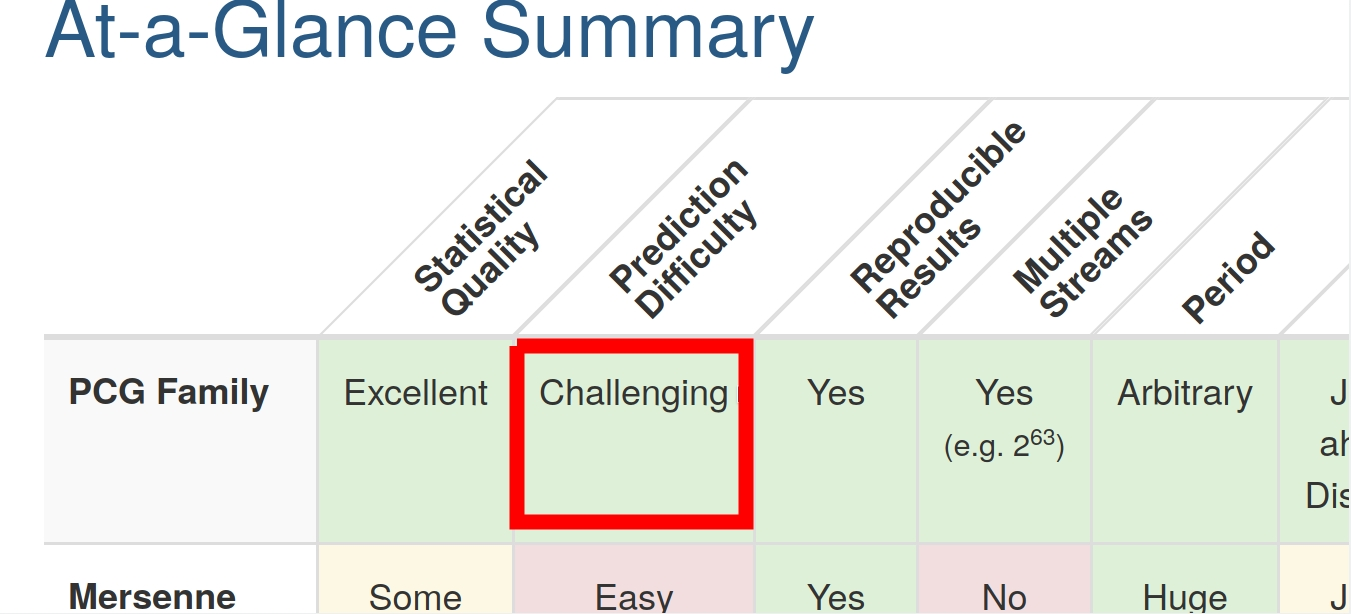
\includegraphics[width=0.9\linewidth]{pictures/PCG_challenging.jpg}
\end{frame}

\begin{frame}
    \centering
    
\includegraphics[height=\textheight]{pictures/accepted.jpg}
\end{frame}

\againframe<2>{intro}

\begin{frame}{Permuted Congruential Generators (\textsf{PCG})}
    \begin{itemize}
        \item Conventional (non-crypto) pseudo-random generators
        \item Designed in 2014 by Melissa O'Neil
        \item \textsf{PCG64}
        \begin{itemize}
            \item Internal state : 128-bit state and 128-bit \alert{increment}
            \item 64-bit outputs
            \item 256-bit seed (or 128-bit with default increment)
            \item Default pseudo-random generator in \textsf{NumPy}
        \end{itemize}
    \end{itemize}

    \begin{center}
    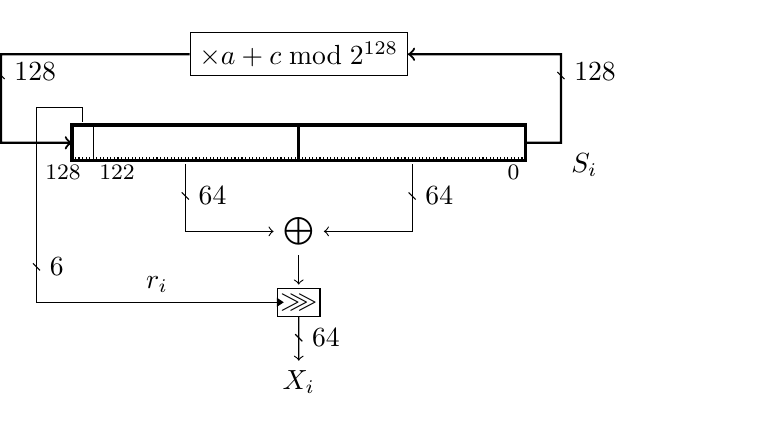
\begin{tikzpicture}[scale=0.45]
      \path[red, use as bounding box] (-1.25, -6.75) rectangle (18.8, 3.75);
      
      % S_i
    
        % bordures
        \draw[very thick]  (0, 0) rectangle (12.8, 1);
        \draw<4->  (0.6, 0) rectangle +(0, 1);
        \draw<3->[very thick]  (6.4, 0) rectangle +(0, 1);
        \foreach \i in {0, 1, ..., 128} \draw (\i/10, 0) -- +(0, 0.1);
        
        % déco autour
        \node<2->[draw] at (6.4, 3) (update) {$\times a + \alert{c} \bmod 2^{128}$};
        \draw<2->[thick,->] (12.8, 0.5) -- (13.8, 0.5) node[below right] {$S_i$} -- (13.8, 3) -- (update);
        \draw<2-> (13.7, 2.5) -- +(0.2, -0.2);
        \path<2-> (13.9, 2.5) node[anchor=west] {128};
        \draw<2->[thick,->] (update) -- (-2, 3) -- (-2, 0.5) node[below left] {$S_{i+1}$} -- (0, 0.5);
        \draw<2-> (-2.1, 2.5) -- +(0.2, -0.2);
        \path<2-> (-1.9, 2.5) node[anchor=west] {128};
    
        
        \node[font=\footnotesize,anchor=east] at (12.9, -0.33) {0};
        %\node<3->[font=\footnotesize,anchor=east] at (6.5, -0.33) {64};
        \node<4->[font=\footnotesize,anchor=west] at (0.5, -0.33) {122};
        \node[font=\footnotesize] at (-0.25, -0.33) {128};
        
        \draw<3-> (6.4, -2) node (x) {$\bigoplus$};
        
        \draw<3->[->] (3.2, -0.1) |- (x);
        \draw<3-> (3.1, -0.9) -- +(0.2, -0.2);
        \path<3-> (3.3, -1) node[anchor=west] {64};
        
        \draw<3->[->] (9.6, -0.1) |- (x);
        \draw<3-> (9.5, -0.9) -- +(0.2, -0.2);
        \path<3-> (9.7, -1) node[anchor=west] {64};
    
        \node<4>[minimum width=1.8cm] at (6.4, -4) (r) {$\ggg$};
        \draw<4> (5.8, -3.6) rectangle +(1.2, -0.8);
        \draw<4>[fill=black] (5.8, -4.1) -- (5.95, -4) -- (5.8, -3.9) -- cycle;
        
        \draw<4> (0.3, 1.1) -- (0.3, 1.5) -- (-1, 1.5) -- (-1, -4) -- node[above] {$r_i$} (5.8, -4);
        \draw<4> (-1.1, -2.9) -- +(0.2, -0.2);
        \path<4> (-0.9, -3) node[anchor=west] {6};
    
        \draw<3->[->] (x) -- +(0, -1.5);
        \node<4> at (6.4, -6.25) (xi) {$X_i$};
        \draw<4>[->] (6.4, -4.4) -- (xi);
    
        \draw<4> (6.3, -4.9) -- +(0.2, -0.2);
        \path<4> (6.5, -5) node[anchor=west] {64};
      \end{tikzpicture}
    \end{center}

  \end{frame}


%%% Local Variables:
%%% mode: latex
%%% TeX-master: "../main"
%%% End:



\section{PCG generators}
\begin{frame}{Attack Outline}

\begin{itemize}
    \item \textbf{Guess} some bits in a few successive states.
    \begin{itemize}
          \item<2-> Least-significant bits
          \item<2-> Rotations
    \end{itemize}
      
    \medskip
      
    \item[$\Rightarrow$] Turn it into a \textbf{(regular) truncated congruential generator}.
      
    \medskip

    \item \textbf{Reconstruct} hidden information using lattice techniques.
    \begin{itemize}
          \item<3-> Easy case: full state
          \item<3-> Hard case: partial information (next rotations)
      \end{itemize}
    
    \medskip
    
    \item \textbf{Discard} bad guesses.
\end{itemize}
\end{frame}



\begin{frame}{Easy Case: Known increment}

If the \alert{increment} (\alert{c}) is \textbf{known}...

\bigskip

\begin{exampleblock}{... Get rid of it!}
\begin{itemize}
    \item $S'_0 \gets S_0$
    \item $S'_1 \gets S_1 - c$
    \item $S'_2 \gets S_2 - (a+1)c$
    \item $S'_3 \gets S_3 - (a^2 + a + 1)c$
    \item $\vdots$
\end{itemize}
\end{exampleblock}

\bigskip

Yields $S' :$ sequence of states with $c=0$ (geometric sequence).

\end{frame}



\begin{frame}[label=atk_details]{Attack Details}

\begin{figure}
\begin{center}
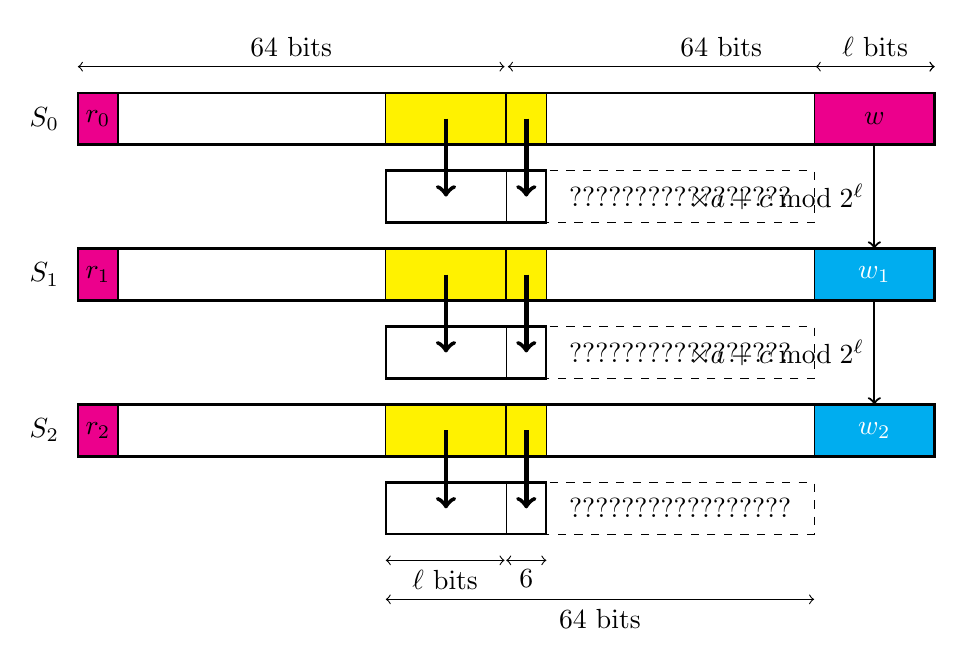
\begin{tikzpicture}[xscale=0.85, yscale=0.66]
  \path[red, use as bounding box] (-0.75, -9.5) rectangle (12.8, 2.25);
  
  % S_0
  \begin{scope}
    % remplissage
    \fill<4-5>[fill=yellow] (4.6, 0) rectangle +(2.4, 1);
    \fill<2-5>[fill=magenta] (0, 0) rectangle node {$r_0$} +(0.6, 1);
    \fill<2-5>[fill=magenta] (11, 0) rectangle node {$w$} +(1.8, 1);
    
    % bordures
    \draw<1-5>[thick]  (0, 0) rectangle (12.8, 1);
    \draw<2-5>  (0.6, 0) rectangle +(0, 1);
    \draw<1-5>[thick]  (6.4, 0) rectangle +(0, 1);
    \draw<4-5>  (7.0, 0) rectangle +(0, 1);
    \draw<4-5> (4.6, 0) rectangle +(0, 1);
    \draw<2-5>  (11, 0) rectangle +(0, 1);
    
    % déco autour
    \node<1-5> at (-0.5, 0.5) {$S_0$};
    \draw<1-5>[<->] (0, 1.5) -- node[above] {64 bits} +(6.375, 0);
    \draw<1>[<->] (6.425, 1.5) -- node[above] {64 bits} +(6.375, 0);
    \draw<2-5>[<->] (12.8, 1.5) -- node[above] {$\ell$ bits} +(-1.775, 0);
  \end{scope}

  % T_0
  \begin{scope}[xshift=4.6cm, yshift=-1.5cm]    
    \draw<5->[dashed]  (0, 0) rectangle +(6.4, 1);
    \draw<5->[thick]   (0, 0) rectangle +(2.4, 1);
    \draw<5>[]   (1.8, 0) rectangle +(0, 1);
    \path<5->  (2.4, 0) rectangle node {$?????????????????$} (6.4, 1);
  \end{scope}

  % flèches S_i --> T_i
  \draw<5> [ultra thick,->] (5.5, 0.5) -- +(0, -1.5);
  \draw<5> [ultra thick,->] (6.7, 0.5) -- +(0, -1.5);

  
  %%%%%%%%%

  
  % S_1
  \begin{scope}[yshift=-3cm]
    % remplissage
    \fill<4-5>[fill=yellow] (4.6, 0) rectangle +(2.4, 1);
    \fill<2-5>[fill=magenta] (0, 0) rectangle node {$r_1$} +(0.6, 1);
    \fill<3-5>[fill=cyan] (11, 0) rectangle node[text=white] {$w_1$} +(1.8, 1);
    
    % bordures
    \draw<1-5>[thick]  (0, 0) rectangle (12.8, 1);
    \draw<2-5>  (0.6, 0) rectangle +(0, 1);
    \draw<1-5>[thick]  (6.4, 0) rectangle +(0, 1);
    \draw<4-5>  (7.0, 0) rectangle +(0, 1);
    \draw<4-5>  (4.6, 0) rectangle +(0, 1);
    \draw<3-5>  (11, 0) rectangle +(0, 1);
    
    % déco autour
    \node<1-5> at (-0.5, 0.5) {$S_1$};

    % flèches S_i --> T_i
    \draw<5>[ultra thick,->] (5.5, 0.5) -- +(0, -1.5);
    \draw<5>[ultra thick,->] (6.7, 0.5) -- +(0, -1.5);
  \end{scope}

  % T_1
  \begin{scope}[xshift=4.6cm, yshift=-4.5cm]    
    \draw<5->[dashed]  (0, 0) rectangle +(6.4, 1);
    \draw<5->[thick]  (0, 0) rectangle +(2.4, 1);
    \draw<5>[]  (1.8, 0) rectangle +(0, 1);
    \path<5-> (2.4, 0) rectangle node {$?????????????????$} (6.4, 1);
  \end{scope}

  %%%%%%%%%%%%%

  
  % S_2
  \begin{scope}[yshift=-6cm]
    % remplissage
    \fill<4-5>[fill=yellow] (4.6, 0) rectangle +(2.4, 1);
    \fill<2-5>[fill=magenta] (0, 0) rectangle node {$r_2$} +(0.6, 1);
    \fill<3-5>[fill=cyan] (11, 0) rectangle node[text=white] {$w_2$} +(1.8, 1);
    
    % bordures
    \draw<1-5>[thick]  (0, 0) rectangle (12.8, 1);
    \draw<2-5>  (0.6, 0) rectangle +(0, 1);
    \draw<1-5>[thick]  (6.4, 0) rectangle +(0, 1);
    \draw<4-5>  (7.0, 0) rectangle +(0, 1);
    \draw<4-5>  (4.6, 0) rectangle +(0, 1);
    \draw<3-5>  (11, 0) rectangle +(0, 1);
    
    % déco autour
    \node<1-5> at (-0.5, 0.5) {$S_2$};
    
    % flèches S_i --> T_i
    \draw<5>[ultra thick,->] (5.5, 0.5) -- +(0, -1.5);
    \draw<5>[ultra thick,->] (6.7, 0.5) -- +(0, -1.5);
  \end{scope}

  % T_2
  \begin{scope}[xshift=4.6cm, yshift=-7.5cm]    
    \draw<5->[dashed]  (0, 0) rectangle +(6.4, 1);
    \draw<5->[thick]  (0, 0) rectangle +(2.4, 1);
    \draw<5>[]  (1.8, 0) rectangle +(0, 1);
    \path<5-> (2.4, 0) rectangle node {$?????????????????$} (6.4, 1);

    % déco
    \draw<5->[<->] (0, -0.5) -- node[below] {$\ell$ bits} +(1.775, 0);
    \draw<5->[<->] (1.8, -0.5) -- node[below] {6} +(0.6, 0);
    \draw<6->[<->] (0, -1.25) -- node[below] {64 bits} +(6.4, 0);
  \end{scope}

  % flèches w
  \draw<3>[thick,->] (11.9, 0) -- node[left] {$\times a + c \bmod \alert{2^\ell}$} +(0, -2);
  \draw<3>[thick,->] (11.9, -3) -- node[left] {$\times a + c \bmod \alert{2^\ell}$} +(0, -2);
  

\end{tikzpicture}
\end{center}
\end{figure}

\end{frame}

%%%%%%%%%%%%%%

\begin{frame}[label=atk_details]{Remove the ``Constant Component''}

\begin{center}
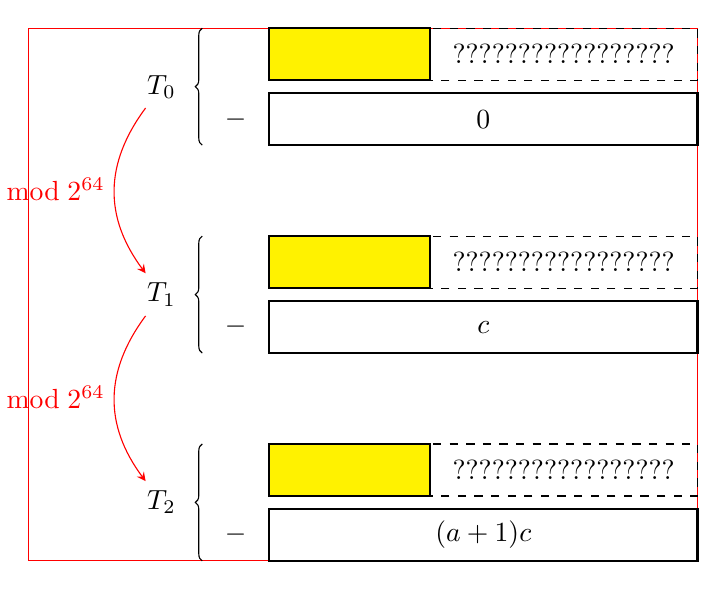
\begin{tikzpicture}[xscale=0.85, yscale=0.66, decoration={brace,mirror},>=stealth]
  \draw[red, use as bounding box] (1, -10.75) rectangle (11, -0.5);
  
  % T_0
  \begin{scope}[xshift=4.6cm, yshift=-1.5cm]    
    \draw[dashed]  (0, 0) rectangle +(6.4, 1);
    \draw[thick,fill=yellow]   (0, 0) rectangle +(2.4, 1);
    %\draw[]   (1.8, 0) rectangle +(0, 1);
    \path  (2.4, 0) rectangle node {$?????????????????$} (6.4, 1);

    % déco
    \draw[decorate]  (-1, 1) -- +(0, -2.25);
    \node[anchor=east] at (-1.25, -0.125)  (T0) {$T_0$};
  \end{scope}

  % composante en c 0
  \begin{scope}[xshift=4.6cm, yshift=-2.75cm]    
  \draw[thick]  (0, 0) rectangle node {$0$} +(6.4, 1);
  \node  at (-0.5, 0.5) {$-$};
  \end{scope}

  % T_1
  \begin{scope}[xshift=4.6cm, yshift=-5.5cm]    
    \draw[dashed]  (0, 0) rectangle +(6.4, 1);
    \draw[thick,fill=yellow]  (0, 0) rectangle +(2.4, 1);
    %\draw[]  (1.8, 0) rectangle +(0, 1);
    \path (2.4, 0) rectangle node {$?????????????????$} (6.4, 1);

    % déco
    \draw[decorate]  (-1, 1) -- +(0, -2.25);
    \node[anchor=east] at (-1.25, -0.125)  (T1) {$T_1$};
  \end{scope}

  % composante en c 1
  \begin{scope}[xshift=4.6cm, yshift=-6.75cm]    
  \draw[thick]  (0, 0) rectangle node {$c$} +(6.4, 1);
  \node  at (-0.5, 0.5) {$-$};
  \end{scope}


  % T_2
  \begin{scope}[xshift=4.6cm, yshift=-9.5cm]    
    \draw[dashed]  (0, 0) rectangle +(6.4, 1);
    \draw[thick,fill=yellow]  (0, 0) rectangle +(2.4, 1);
    %\draw[]  (1.8, 0) rectangle +(0, 1);
    \path (2.4, 0) rectangle node {$?????????????????$} (6.4, 1);

    % déco
    \draw[decorate]  (-1, 1) -- +(0, -2.25);
    \node[anchor=east] at (-1.25, -0.125) (T2) {$T_2$};
  \end{scope}

    % composante en c 2
  \begin{scope}[xshift=4.6cm, yshift=-10.75cm]    
  \draw[thick]  (0, 0) rectangle node {$(a+1)c$} +(6.4, 1);
  \node  at (-0.5, 0.5) {$-$};
  \end{scope}

  
  % arrows
  \draw[red,->] (T0) edge[bend right] node[left] {$\times a \bmod 2^{64}$} (T1);
  \draw[red,->] (T1) edge[bend right] node[left] {$\times a \bmod 2^{64}$} (T2);
  
\end{tikzpicture}
\end{center}

\end{frame}


%%% Local Variables:
%%% mode: latex
%%% TeX-master: "../main.tex"
%%% End:

\begin{frame}<3>{Truncated Linear Congruencial Generators(\textsf{TLCG})}
    \begin{itemize}
            \item Internal state : \(2^k\)-bit state.
            \item Multiplier $a$: known constant.
            \item Initial state: unknown \(2^k\)-bit seed.
    \end{itemize}
    
    \bigskip
    
    \begin{center}
    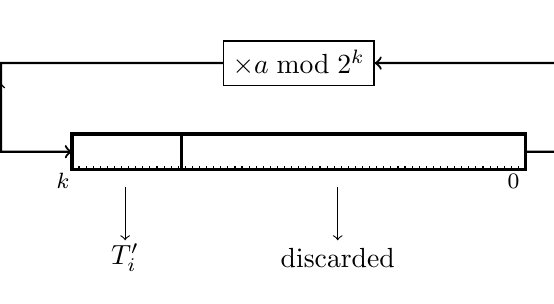
\begin{tikzpicture}[scale=0.45]
      \path[red, use as bounding box] (-1.25, -3) rectangle (12.8, 4);
      
      % S_i
    
        % bordures
        \draw[very thick]  (0, 0) rectangle (12.8, 1);

        \draw<3->[very thick]  (3.1, 0) rectangle +(0, 1);
        \foreach \i in {0, 1, ..., 64} \draw (\i/5, 0) -- +(0, 0.1);
        
        % déco autour
        \node<2->[draw] at (6.4, 3) (update) {$\times a \bmod 2^{k}$};
        \draw<2->[thick,->] (12.8, 0.5) -- (13.8, 0.5) node[below right] {} -- (13.8, 3) -- (update);
        \draw<2-> (13.7, 2.5) -- +(0.2, -0.2);
        \path<2-> (13.9, 2.5);
        \draw<2->[thick,->] (update) -- (-2, 3) -- (-2, 0.5) node[below left] {} -- (0, 0.5);
        \draw<2-> (-2.1, 2.5) -- +(0.2, -0.2);
        \path<2-> (-1.9, 2.5);
    
        
        \node[font=\footnotesize,anchor=east] at (12.9, -0.33) {0};
        %\node<3->[font=\footnotesize,anchor=east] at (6.5, -0.33) {64};
        \node[font=\footnotesize] at (-0.25, -0.33) {$k$};
        

        
 
        \draw<3->[->] (1.5, -0.5) -- (1.5, -2);
        \path<3-> (1.7, -1) ;
        \node<3-> at (1.5,-2.5) {\(T'_i\)};
        
        \draw<3->[->] (7.5, -0.5) -- (7.5, -2);
        \path<3-> (7.7, -1) ;
        \node<3-> at (7.5,-2.5) {discarded};

      \end{tikzpicture}
    \end{center}
    
\end{frame}

\begin{frame}{Reconstructing Truncated Geometric Sequences}

\begin{itemize}
    \item Sequence $u_{i+1} = a \times u_i \bmod 2^k$.
    \item $T$ = Truncated version (low-order bits unknown).
    %\item Reconstruction algorithm: Frieze \textit{et al} (CVP problem)

\item \(\mathcal{L}\) = lattice spawned by the rows of
\[
 \begin{pmatrix}
    1 & a   & a^2 & \dots & a^{n-1} \\
    0 & 2^{k} & 0   & \dots & 0 \\
    0 & 0   & 2^{k} & \dots & 0 \\
    \dots & \dots & \dots & \dots & \dots\\
    0 & 0 & 0 & \dots & 2^{k} \\
  \end{pmatrix}
\]        
%Then $LCG_{n,k}(x,0)\in \mathcal{L}$.
%\medskip
\end{itemize}

\medskip

\begin{block}{Main Idea}
\begin{itemize}
\item $\mathbf{u} = (u_0, u_1, \dots, u_{n-1})$ \textbf{belongs} to the lattice $\mathcal{L}$.
\item $T$ (truncated geometric series) is an \textbf{approximation} of $\mathbf{u}$.
\item[$\Rightarrow$] $T$ is \textbf{close} to a point of $\mathcal{L}$.
\item[$\Rightarrow$] \textbf{Closest} point to $T$ in $\mathcal{L}$ $\leadsto$ $\mathbf{u}$.
\end{itemize}
\end{block}
\end{frame}

%%%%%%%%%%%%%%%%%%%%%%%%%%%%%%%%%%%%%%%%%%%%%%%%

\begin{frame}{\textbf{Lattices and Basis reduction}}
\begin{itemize}
    \item Lattice : subgroup of $\mathbb{R}^n$ isomorphic to $\mathbb{Z}^m$
\end{itemize}
\begin{center}
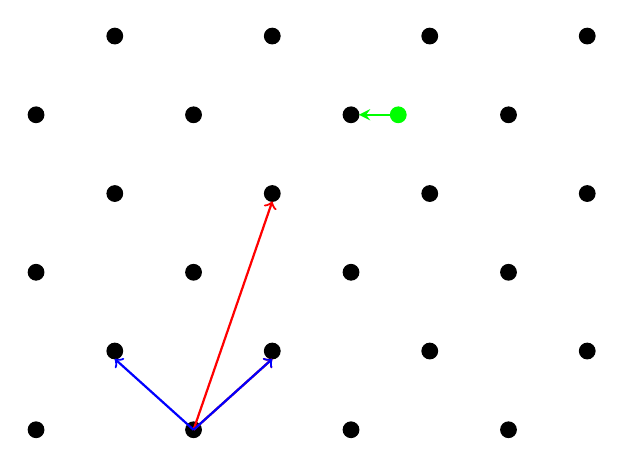
\begin{tikzpicture}

    \foreach \x in {2,3,4,5}{
		\foreach \y in {0,1,2}{
			\node[draw,circle,inner sep=2pt,fill] at (2*\x,2*\y) {};
			\node[draw,circle,inner sep=2pt,fill] at (2*\x+1,2*\y+1) {};
			
		}
	}
    \draw[->,thick,red] (6,0) --(7,2.9);
    \draw[->,thick,red] (6,0) --(7,0.9);
    %\draw[->,dashed,red] (7,3) --(8,3.9);
    %\draw[->,dashed,red] (7,1) --(8,3.9);
    
    \draw<2->[->,thick,blue] (6,0) --(7,0.9);
    \draw<2->[->,thick,blue] (6,0) --(5,0.9);
    %\draw<2->[->,dashed,blue] (5,1) --(6,1.9);
    %\draw<2->[->,dashed,blue] (7,1) --(6,1.9);
    
    \node<3>[draw,circle,inner sep=2pt,green,fill] at (2*4.3, 2*2) {};
    \draw<3>[draw,thick,green,->,>=stealth] (2*4.3, 2*2) -- +(-0.5, 0);
    
\end{tikzpicture}
\end{center}
\pause[2]
\begin{itemize}
    \item The blue basis is \emph{shorter} than the red basis.
    \item LLL algorithm reduces bases in polynomial time.
\end{itemize}
\end{frame}

%%%%%%%%%%%%%%%%%%%%%%%%%%%%%%%%%%%%%%%%%%%%%%%%

\begin{frame}{CVP problem and Babai rounding}
  \begin{alertblock}{Closest Vector Problem}
    \begin{itemize}
    \item Standard \textbf{NP-hard} problem on lattices.
    \item Given arbitrary $\mathbf{x} \in \mathbb{Z}^n$, find closest lattice point.
  \end{itemize}
\end{alertblock}

\medskip

\begin{block}{Babai Rounding Algorithm}
      \begin{itemize}
      \item Approximately solves CVP.
        \[
          BabaiRounding(\mathbf{x}, \mathcal{L}) = H\times \mathrm{round}\left(H^{-1}\times \mathbf{x}\right)
        \]
        Where \(H\) is a ``good'' (LLL-reduced) basis of the lattice $\mathcal{L}$.

      \item FAST (two matrix-vector products + rounding)
      \item Exponentially bad approximation (in the lattice dimension).
      \item[$\rightarrow$] Often exact in small dimension though.
      \end{itemize}
    \end{block}    
\end{frame}



%%% Local Variables:
%%% mode: latex
%%% TeX-master: "../main"
%%% End:


\section{Case with known increment (easy)}
\begin{frame}{Implementation (Easy case, known increment)}
  \begin{block}{Summary}
    \begin{itemize}
    \item Observe 3 outputs $X_0, X_1, X_2$ (192 bits).
    \item Guess 37 bits:
      \begin{itemize}
      \item \(n=3\) successive rotations (6 bits each),
      \item \(\ell=19\) least significant bits of \(S_0\),
      \end{itemize}
    \item Solve \(2^{37}\) instances of CVP in dimension 3 (Babai Rounding).
    \item Reconstruct initial state, check outputs.
    \end{itemize}
  \end{block}

  \begin{alertblock}{Caveat}
    Attack proved correct for $\ell=20$, works fine for $\ell=19$...
  \end{alertblock}
  
  \begin{exampleblock}{Concretely...}
    \begin{itemize}
    \item $25$ CPU cycles per guess, 23 CPU-minutes in total.
    \end{itemize}
  \end{exampleblock}  
\end{frame}


%%% Local Variables:
%%% mode: latex
%%% TeX-master: "../main"
%%% End:


\section{Case with unknown increment (hard)}

\begin{frame}[label=hard]{Issue with $c$ unknown}

  \begin{exampleblock}{Summary so far (the \textbf{Easy Case})}
    \begin{itemize}
    \item The \alert{increment} (\alert{c}) is \textbf{known}:
      \begin{itemize}
      \item Remove it, get truncated geometric sequence, CVP.
      \end{itemize}
    \end{itemize}
  \end{exampleblock}
  
  \begin{alertblock}{Now the \textbf{Hard Case}}
    \begin{itemize}
    \item The \alert{increment} (\alert{c}) is \textbf{unknown}:
      \begin{itemize}
      \item How to get truncated geometric sequence?
      \item Use $\Delta S_i = S_{i+1} - S_i \qquad\qquad (\Delta S_{i+1} = a \times \Delta S_i \bmod 2^{128})$.
      \end{itemize}
      \pause
    \item Same attack as before, but...
      \begin{itemize}
    \item Must guess one more rotation.
    \item Must guess least-significant bits of \alert{$c$}.
    \end{itemize}
  \end{itemize}
  \end{alertblock}
\end{frame}

%%%%%%%%%%%%%%%%%%%%%%%%%%%%%%%%%%%%%%%%%%%%%%%%%%%%%%%%%%%%%


\begin{frame}[label=hard_dtl]{Attack Details}

\begin{figure}
\begin{center}
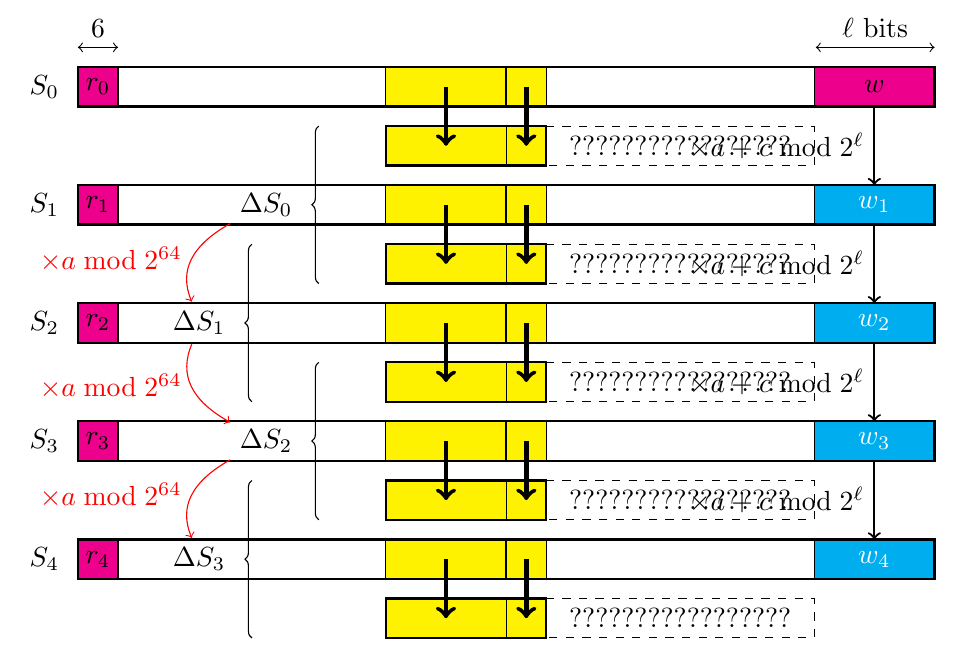
\begin{tikzpicture}[xscale=0.85, yscale=0.5]
  \path[red, use as bounding box] (-0.75, -13.5) rectangle (12.8, 2);
  
  % S_0
  \begin{scope}
    % remplissage
    \fill<4-5>[fill=yellow] (4.6, 0) rectangle +(2.4, 1);
    \fill<2-5>[fill=magenta] (0, 0) rectangle node {$r_0$} +(0.6, 1);
    \fill<2-5>[fill=magenta] (11, 0) rectangle node {$w$} +(1.8, 1);
    
    % bordures
    \draw<1-5>[thick]  (0, 0) rectangle (12.8, 1);
    \draw<2-5>  (0.6, 0) rectangle +(0, 1);
    \draw<1-5>[thick]  (6.4, 0) rectangle +(0, 1);
    \draw<4-5>  (7.0, 0) rectangle +(0, 1);
    \draw<4-5> (4.6, 0) rectangle +(0, 1);
    \draw<2-5>  (11, 0) rectangle +(0, 1);
    
    % déco autour
    \node<1-5> at (-0.5, 0.5) {$S_0$};
    \draw<2-5>[<->] (12.8, 1.5) -- node[above] {$\ell$ bits} +(-1.775, 0);
    \draw<2-5>[<->] (0, 1.5) -- node[above] {6} +(0.6, 0);
  \end{scope}

  % T_0
  \begin{scope}[xshift=4.6cm, yshift=-1.5cm]    
    \draw<5->[dashed]  (0, 0) rectangle +(6.4, 1);
    \draw<5->[thick,fill=yellow]   (0, 0) rectangle +(2.4, 1);
    \draw<5>[]   (1.8, 0) rectangle +(0, 1);
    \path<5->  (2.4, 0) rectangle node {$?????????????????$} (6.4, 1);
  \end{scope}

  % flèches S_i --> T_i
  \draw<5> [ultra thick,->] (5.5, 0.5) -- +(0, -1.5);
  \draw<5> [ultra thick,->] (6.7, 0.5) -- +(0, -1.5);

  
  %%%%%%%%%

  
  % S_1
  \begin{scope}[yshift=-3cm]
    % remplissage
    \fill<4-5>[fill=yellow] (4.6, 0) rectangle +(2.4, 1);
    \fill<2-5>[fill=magenta] (0, 0) rectangle node {$r_1$} +(0.6, 1);
    \fill<3-5>[fill=cyan] (11, 0) rectangle node[text=white] {$w_1$} +(1.8, 1);
    
    % bordures
    \draw<1-5>[thick]  (0, 0) rectangle (12.8, 1);
    \draw<2-5>  (0.6, 0) rectangle +(0, 1);
    \draw<1-5>[thick]  (6.4, 0) rectangle +(0, 1);
    \draw<4-5>  (7.0, 0) rectangle +(0, 1);
    \draw<4-5>  (4.6, 0) rectangle +(0, 1);
    \draw<3-5>  (11, 0) rectangle +(0, 1);
    
    % déco autour
    \node<1-5> at (-0.5, 0.5) {$S_1$};
  \end{scope}
  
  % T_1
  \begin{scope}[xshift=4.6cm, yshift=-4.5cm]    
    \draw<5->[dashed]  (0, 0) rectangle +(6.4, 1);
    \draw<5->[thick,fill=yellow]  (0, 0) rectangle +(2.4, 1);
    \draw<5>[]  (1.8, 0) rectangle +(0, 1);
    \path<5-> (2.4, 0) rectangle node {$?????????????????$} (6.4, 1);
  \end{scope}

  \begin{scope}[yshift=-3cm]
    % flèches S_i --> T_i
    \draw<5>[ultra thick,->] (5.5, 0.5) -- +(0, -1.5);
    \draw<5>[ultra thick,->] (6.7, 0.5) -- +(0, -1.5);
  \end{scope}

  
  %%%%%%%%%%%%%

  
  % S_2
  \begin{scope}[yshift=-6cm]
    % remplissage
    \fill<4-5>[fill=yellow] (4.6, 0) rectangle +(2.4, 1);
    \fill<2-5>[fill=magenta] (0, 0) rectangle node {$r_2$} +(0.6, 1);
    \fill<3-5>[fill=cyan] (11, 0) rectangle node[text=white] {$w_2$} +(1.8, 1);
    
    % bordures
    \draw<1-5>[thick]  (0, 0) rectangle (12.8, 1);
    \draw<2-5>  (0.6, 0) rectangle +(0, 1);
    \draw<1-5>[thick]  (6.4, 0) rectangle +(0, 1);
    \draw<4-5>  (7.0, 0) rectangle +(0, 1);
    \draw<4-5>  (4.6, 0) rectangle +(0, 1);
    \draw<3-5>  (11, 0) rectangle +(0, 1);
    
    % déco autour
    \node<1-5> at (-0.5, 0.5) {$S_2$};
  \end{scope}    
  
  % T_2
  \begin{scope}[xshift=4.6cm, yshift=-7.5cm]    
    \draw<5->[dashed]  (0, 0) rectangle +(6.4, 1);
    \draw<5->[thick,fill=yellow]  (0, 0) rectangle +(2.4, 1);
    \draw<5>[]  (1.8, 0) rectangle +(0, 1);
    \path<5-> (2.4, 0) rectangle node {$?????????????????$} (6.4, 1);
  \end{scope}

  \begin{scope}[yshift=-6cm]
    % flèches S_i --> T_i
    \draw<5>[ultra thick,->] (5.5, 0.5) -- +(0, -1.5);
    \draw<5>[ultra thick,->] (6.7, 0.5) -- +(0, -1.5);
  \end{scope}

  
  %%%%%%%%%%%%%

  
  % S_3
  \begin{scope}[yshift=-9cm]
    % remplissage
    \fill<4-5>[fill=yellow] (4.6, 0) rectangle +(2.4, 1);
    \fill<2-5>[fill=magenta] (0, 0) rectangle node {$r_3$} +(0.6, 1);
    \fill<3-5>[fill=cyan] (11, 0) rectangle node[text=white] {$w_3$} +(1.8, 1);
    
    % bordures
    \draw<1-5>[thick]  (0, 0) rectangle (12.8, 1);
    \draw<2-5>  (0.6, 0) rectangle +(0, 1);
    \draw<1-5>[thick]  (6.4, 0) rectangle +(0, 1);
    \draw<4-5>  (7.0, 0) rectangle +(0, 1);
    \draw<4-5>  (4.6, 0) rectangle +(0, 1);
    \draw<3-5>  (11, 0) rectangle +(0, 1);
    
    % déco autour
    \node<1-5> at (-0.5, 0.5) {$S_3$};
   \end{scope}

  % T_3
  \begin{scope}[xshift=4.6cm, yshift=-10.5cm]    
    \draw<5->[dashed]  (0, 0) rectangle +(6.4, 1);
    \draw<5->[thick,fill=yellow]  (0, 0) rectangle +(2.4, 1);
    \draw<5>[]  (1.8, 0) rectangle +(0, 1);
    \path<5-> (2.4, 0) rectangle node {$?????????????????$} (6.4, 1);
  \end{scope}

  \begin{scope}[yshift=-9cm]
  % flèches S_i --> T_i
    \draw<5>[ultra thick,->] (5.5, 0.5) -- +(0, -1.5);
    \draw<5>[ultra thick,->] (6.7, 0.5) -- +(0, -1.5);
  \end{scope}
  
    %%%%%%%%%%%%%

  
  % S_4
  \begin{scope}[yshift=-12cm]
    % remplissage
    \fill<4-5>[fill=yellow] (4.6, 0) rectangle +(2.4, 1);
    \fill<2-5>[fill=magenta] (0, 0) rectangle node {$r_4$} +(0.6, 1);
    \fill<3-5>[fill=cyan] (11, 0) rectangle node[text=white] {$w_4$} +(1.8, 1);
    
    % bordures
    \draw<1-5>[thick]  (0, 0) rectangle (12.8, 1);
    \draw<2-5>  (0.6, 0) rectangle +(0, 1);
    \draw<1-5>[thick]  (6.4, 0) rectangle +(0, 1);
    \draw<4-5>  (7.0, 0) rectangle +(0, 1);
    \draw<4-5>  (4.6, 0) rectangle +(0, 1);
    \draw<3-5>  (11, 0) rectangle +(0, 1);
    
    % déco autour
    \node<1-5> at (-0.5, 0.5) {$S_4$};
  \end{scope}    

  % T_4
  \begin{scope}[xshift=4.6cm, yshift=-13.5cm]    
    \draw<5->[dashed]  (0, 0) rectangle +(6.4, 1);
    \draw<5->[thick,fill=yellow]  (0, 0) rectangle +(2.4, 1);
    \draw<5>[]  (1.8, 0) rectangle +(0, 1);
    \path<5-> (2.4, 0) rectangle node {$?????????????????$} (6.4, 1);
  \end{scope}
  \begin{scope}[yshift=-12cm]
  % flèches S_i --> T_i
    \draw<5>[ultra thick,->] (5.5, 0.5) -- +(0, -1.5);
    \draw<5>[ultra thick,->] (6.7, 0.5) -- +(0, -1.5);
  \end{scope}

  
  % Differences
  \begin{scope}[xshift=4.6cm, decoration={brace,mirror},>=stealth]  
    \draw<6>[decorate]  (-1, -0.5) -- +(0, -4);
    \node<6>[anchor=east] at (-1.25, -2.5)  (T0) {$\Delta S_0$};
  \end{scope}

  % Differences
  \begin{scope}[xshift=3.6cm, yshift=-3cm, decoration={brace,mirror},>=stealth]  
    \draw<6>[decorate]  (-1, -0.5) -- +(0, -4);
    \node<6>[anchor=east] at (-1.25, -2.5)  (T1) {$\Delta S_1$};
  \end{scope}

  % Differences
  \begin{scope}[xshift=4.6cm, yshift=-6cm, decoration={brace,mirror},>=stealth]  
    \draw<6>[decorate]  (-1, -0.5) -- +(0, -4);
    \node<6>[anchor=east] at (-1.25, -2.5)  (T2) {$\Delta S_2$};
  \end{scope}

  % Differences
  \begin{scope}[xshift=3.6cm, yshift=-9cm, decoration={brace,mirror},>=stealth]  
    \draw<6>[decorate]  (-1, -0.5) -- +(0, -4);
    \node<6>[anchor=east] at (-1.25, -2.5)  (T3) {$\Delta S_3$};
  \end{scope}

  % arrows
  \draw<6>[red,->] (T0) edge[bend right] node[left] {$\times a \bmod 2^{64}$} (T1);
  \draw<6>[red,->] (T1) edge[bend right] node[left] {$\times a \bmod 2^{64}$} (T2);
  \draw<6>[red,->] (T2) edge[bend right] node[left] {$\times a \bmod 2^{64}$} (T3);

  % flèches w
  \draw<3>[thick,->] (11.9, 0) -- node[left] {$\times a + c \bmod \alert{2^\ell}$} +(0, -2);
  \draw<3>[thick,->] (11.9, -3) -- node[left] {$\times a + c \bmod \alert{2^\ell}$} +(0, -2);
  \draw<3>[thick,->] (11.9, -6) -- node[left] {$\times a + c \bmod \alert{2^\ell}$} +(0, -2);
  \draw<3>[thick,->] (11.9, -9) -- node[left] {$\times a + c \bmod \alert{2^\ell}$} +(0, -2);
  
\end{tikzpicture}
\end{center}
\end{figure}
\end{frame}

%%%%%%%%%%%%%%%%%%%%%%%%%%%%%%%%%%%%%%%%%%%%%%%%%%%%%%%%%%%%

\begin{frame}<1>[label=hard_test]{Attack Details (cont'd)}

  \begin{block}{Summary so far}
    \begin{itemize}
    \item \textbf{Guess} parts of the states ($S_i$).
    \item Attack state \textbf{differences} ($\Delta S_i$).
    \item CVP in dim. 4 $\leadsto$ reconstruct partial $\Delta S_i \qquad$ (for all $i$).
    \end{itemize}
  \end{block}

  \bigskip

  \begin{alertblock}{Problem}
    How to check if guesses are valid?
  \end{alertblock}

  \bigskip
  \pause

  \begin{exampleblock}{Solution}
    \begin{itemize}
    \item $\color{cyan} S_i[64:64+\ell]$ from guesses + $X_i$ (output) + $r_i$ (rotation).
    \item $\color{orange} S_i[64:64+\ell]$ from guesses + partial $\Delta S_i$.
    \item[$\Rightarrow$] Try all possible $r_i$'s. No match $\leadsto$ bad guess.
    \end{itemize}
  \end{exampleblock}
\end{frame}


%%%%%%%%%%%%%%%%%%%%%%%%%%%%%%%%%%%%%%%%%%%%%%%%%%%%%%%%%%%%

\begin{frame}[label=hard_test_dtl]{Consistency Check}

%  For any future state $S_i$:
  
  %for $0 \leq r \leq 63$
    \begin{center}
    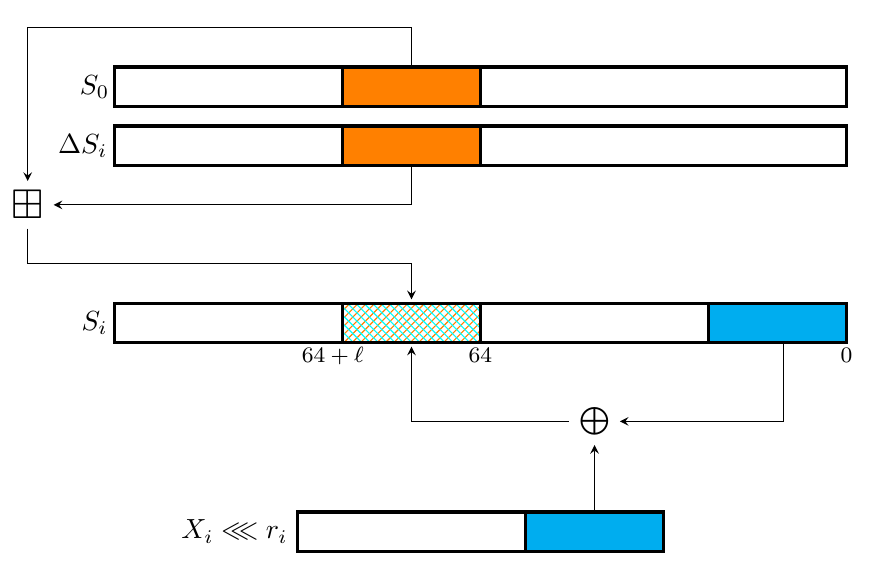
\begin{tikzpicture}[scale=0.5,>=stealth]
      \path[red, use as bounding box] (-8, -6.5) rectangle (12.8, 7);

      % S_0
      \node<2-> at (-6.3, 5.5) {$S_0$};
      \draw<2->[very thick]  (-5.8, 5) rectangle +(18.6, 1);
      \draw<2->[very thick,fill=orange] (0, 5) rectangle +(3.5, 1);

      % Delta S_i
      \node<2-> at (-6.6, 4) {$\Delta S_i$};
      \draw<2->[very thick]  (-5.8, 3.5) rectangle +(18.6, 1);
      \draw<2->[very thick,fill=orange] (0, 3.5) rectangle +(3.5, 1);


      \node<3-> at (-8, 2.5) (add) {\scalebox{1.5}{$\boxplus$}};
      \draw<3->[->] (1.75, 6) -- (1.75, 7) -- (-8, 7) -- (add);
      \draw<3->[->] (1.75, 3.5) -- (1.75, 2.5) -- (add);
      \draw<3->[->] (add) -- (-8, 1) -- (1.75, 1) -- (1.75, 0.1);

      \begin{scope}[yshift=-1cm]
      
        % S_i
        \node at (-6.3, 0.5) {$S_i$};
        \draw[very thick]  (-5.8, 0) rectangle +(18.6, 1);
        \fill<3->[pattern=north east lines, pattern color=orange] (0, 0) rectangle +(3.5, 1);
        \fill<5->[pattern=north west lines, pattern color=cyan]   (0, 0) rectangle +(3.5, 1);
        \draw[very thick] (0, 0) rectangle +(3.5, 1);
        \draw<4->[very thick,fill=cyan] (9.3, 0) rectangle (12.8, 1);
        
        \node[font=\footnotesize] at (12.8, -0.33) {$0$};
        \node[font=\footnotesize] at (3.5, -0.33) {$64$};
        
        \node[font=\footnotesize] at (-0.25, -0.33) {$64 +\ell$ };
%        \node[font=\footnotesize] at (-6, -0.33) {$128$};
        
        \draw<5-> (6.4, -2) node (x) {$\bigoplus$};
        
        \draw<5->[<-] (1.75, -0.1) |- (x);
        \draw<5->[->] (11.2, -0.0) |- (x);
        \draw<5->[<-] (x) --  (6.4, -4.3);
        
        % X_i
        \begin{scope}[xshift=-1.15cm]
        \node<4->[anchor=east] at (0, -4.8) {$X_i \lll r_i$};
        \draw<4->[very thick]  (0, -4.3) rectangle +(9.3, -1);
        \draw<4->[very thick,fill=cyan]  (9.3, -4.3) rectangle +(-3.5, -1);
      \end{scope}
    \end{scope}
  \end{tikzpicture}
    \end{center}
\end{frame}

\againframe<2>{hard_test}

% \begin{frame}{Complete State Reconstruction}
% \begin{itemize}
%     \item We get the Full Difference:
%     \begin{itemize}
%         \item We recover the 63 first rotations
%         \item $\Delta S_i[122:128] = r_{i+1} - r_{i}$
%         \item $\Delta S = CVP(2^{122} \Delta S[122:128],\mathcal{L})$
%     \end{itemize}
%     \item  We deduce the entire $S_0$
%     \begin{itemize}
%         \item probably could have used a SAT-solver
%         \item we recover $S_0$ from right to left by computing the carries
%     \end{itemize}
% \end{itemize}
% \end{frame}


%%%%%%%%%%%%%%%%%%%%%%%%%%%%%%%%%%%%%%%%%%%%%%%%%%%%%%%%%%%%

\begin{frame}<1>[label=hard_finish]{Finishing it Off}

  \begin{block}{Summary so far}
    \begin{itemize}
    \item \textbf{Guessed} parts of the states ($S_i$).
    \item Isolated \textbf{correct} guess $\leadsto$ correct partial differences $\Delta S_i$.
    \end{itemize}
  \end{block}

  \bigskip

  \begin{alertblock}{Problem}
    How to get full initial state $S_0$?
  \end{alertblock}

  \bigskip
  \pause

  \begin{exampleblock}{Solution}
    \begin{itemize}
    \item Correct partial $\Delta S_i$ + consistency check $\leadsto$ \textbf{all} rotations $r_i$.
    \item[$\Rightarrow$] MSB of all $S_i$ $\leadsto$ MSB of all $\Delta S_i$.
    \item[$\Rightarrow$] CVP in dim. 64 $\leadsto$ full $\Delta S_0$.
      \pause
    \item The rest is easy.
    \end{itemize}
  \end{exampleblock}
\end{frame}


\againframe<5>{hard_test_dtl}
\againframe<2>{hard_finish}


\begin{frame}[label=hard_big_cvp]{Reconstructing the Full Differences (CVP in dim. 64)}
  \begin{center}
    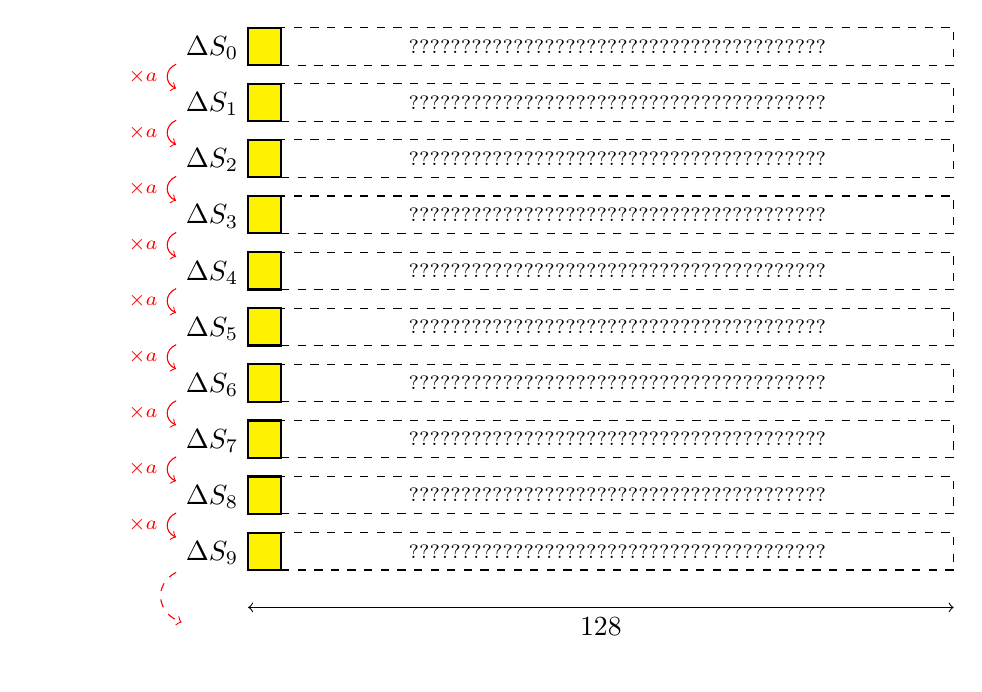
\begin{tikzpicture}[xscale=0.7, yscale=0.475]
      \path[red, use as bounding box] (-4, -16) rectangle (12.8, 1);
      
      
      % T_0
      \foreach \i in {0, 1, ..., 9} {
        \begin{scope}[yshift=-\i*1.5cm]    
          \draw[dashed]  (0, 0) rectangle +(12.8, 1);
          \draw[thick,fill=yellow]  (0, 0) rectangle +(0.6, 1);
          \path (0.6, 0) rectangle node[font=\scriptsize] {$????????????????????????????????????????$} (12.8, 1);
          \node [anchor=east] at (0, 0.45) (DS_\i) {$\Delta S_{\i}$};
        \end{scope}
      }
      
        \begin{scope}[yshift=-10.5*1.5cm]    
          \node [anchor=east] at (0.3, 0.45) (DS_10) {\phantom{$\Delta S_{11}$}};
        \end{scope}

      
      % arrows
      \draw[red,->] (DS_0) edge[bend right=2cm] node[left,font=\scriptsize] {$\times a$} (DS_1);
      \draw[red,->] (DS_1) edge[bend right=2cm] node[left,font=\scriptsize] {$\times a$} (DS_2);
      \draw[red,->] (DS_2) edge[bend right=2cm] node[left,font=\scriptsize] {$\times a$} (DS_3);
      \draw[red,->] (DS_3) edge[bend right=2cm] node[left,font=\scriptsize] {$\times a$} (DS_4);
      \draw[red,->] (DS_4) edge[bend right=2cm] node[left,font=\scriptsize] {$\times a$} (DS_5);
      \draw[red,->] (DS_5) edge[bend right=2cm] node[left,font=\scriptsize] {$\times a$} (DS_6);
      \draw[red,->] (DS_6) edge[bend right=2cm] node[left,font=\scriptsize] {$\times a$} (DS_7);
      \draw[red,->] (DS_7) edge[bend right=2cm] node[left,font=\scriptsize] {$\times a$} (DS_8);
      \draw[red,->] (DS_8) edge[bend right=2cm] node[left,font=\scriptsize] {$\times a$} (DS_9);
      \draw[red,->,dashed] (DS_9) edge[bend right=2cm] (DS_10);

      % size
      \draw[<->] (0, -14.5) -- node[below] {128} +(12.8, 0);
    \end{tikzpicture}
  \end{center}
\end{frame}

\againframe<3>{hard_finish}

%%% Local Variables:
%%% mode: latex
%%% TeX-master: "../main"
%%% End:


\section{Conclusion}
\begin{frame}[label=bragging]{Implementation (Hard case, unknown increment)}
  \begin{block}{Summary}
    \begin{itemize}
    \item Guess $k=$51--55 bits:
      \begin{itemize}
      \item $n=5$ successive rotations (6 bits each),
      \item $\ell=$ 11--13 least significant bits of \(S_0\) \textbf{and} \alert{$c$}.
      \end{itemize}
    \item Solve \(2^{k}\) instances of CVP in dimension 4 (Babai Rounding).
    \item Consistency Check.
    \end{itemize}
  \end{block}

  \begin{alertblock}{Caveat}
    \begin{itemize}
    \item Attack proved correct for $\ell=14$.
    \item Works fine for $\ell=13$.
    \item OK with $p=0.66$ with $\ell=11$.
    \end{itemize}
  \end{alertblock}
  
  \begin{exampleblock}{Concretely...}
    \begin{itemize}
    \item $55$ CPU cycles per guess, 12.5k--20k CPU-hours in total.
    \end{itemize}
  \end{exampleblock}
\end{frame}

%%%%%%%%%%%%%%%%%%%%%%%%

\begin{frame}[label=bragging]{Doing it for Real}
  \begin{center}
    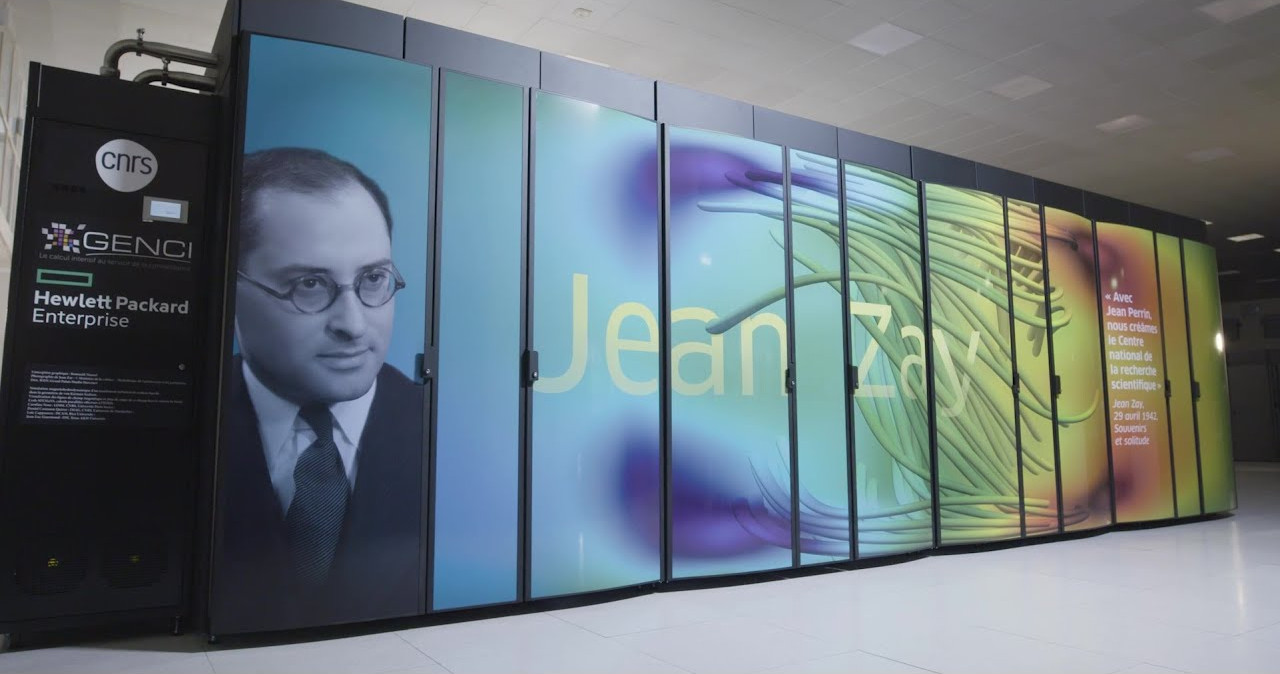
\includegraphics[width=0.7\linewidth]{pictures/Jean_Zay.jpg}
  \end{center}

  \begin{itemize}
    \item Nodes: 2$\times$ 20-cores \textsf{Intel Xeon Gold 6248 @ 2.5Ghz}, ``\emph{Cascade Lake}''
    \item Running time: 35 minutes on 512 nodes.
    \item Complete recovery using 512 consecutive output bytes.
    \end{itemize}
    
\end{frame}
%%% Local Variables:
%%% mode: latex
%%% TeX-master: "../main"
%%% End:


\end{document}


%%% Local Variables:
%%% TeX-command-extra-options: "-shell-escape"
%%% ispell-local-dictionary: "english"
%%% eval: (flyspell-mode 1)
%%% eval: (reftex-mode 1)
%%% End:
